\documentclass{article}
\usepackage{amsmath}
\usepackage{amsfonts}
\usepackage[english]{babel}
\usepackage[utf8]{inputenc}
\usepackage{amsthm}
\usepackage{graphicx}
\usepackage{array}
\usepackage{tabularx}

\newcommand{\norm}[1]{\left\lVert#1\right\rVert}
\newtheorem{theorem}{Theorem}
\newtheorem{prop}{Proposition}

\begin{document}

\title{Parallel Processing Homework 2}
\author{Toby Harvey}
\maketitle


In this homework I implemented 2 different algorithms for doing a prefix sum on a length $n$ vector. The first algorithm could run in $O(\log n)$ time if $n$ processors were available, although this is a very unrealistic assumption for large arrays, making the inner loop in which sums are updated (see lines 149, and 161 of prefix.c) run at $\frac{n}{\# \text{processors}}$. Another disadvantage of the first method is that the sum cannot be computed in place (after its copied out of the original array), because there are many possibilities for one thread to overwrite data needed by a behind thread. I used two arrays one to write to and one to read to to avoid this problem, but this adds another $\frac{n}{\# \text{processors}}$ computations for the copying to prepare for the next iteration (see line 161 in prefix.c). This doesn't affect the $O$ time complexity but it does add some time.

I ran the 3 implementations on talapas with 28 core Intel Xeon dual E5-2690v4. In the first plot I ran the code with a fixed number of elements $1024$, and we see what looks like a logarithmic decay. Noting that since we have 28 core's and never more than 28 threads there should never be any thread scheduling overhead or wait times for threads, so the decreasing marginal returns cannot be attributed to this. I believe the simple answer to this logarithmic shape is that the benefit of, for instance, going from splitting an array into 2 pieces to be done in parallel to 3, has a much greater effect than going from an array in 20 pieces to 21 pieces in parallel. It is also interesting that the number of threads has such a drastic effect on the $N\log(N)$ algorithm compared to the parallel $N$ algorithm. One possible explanation for this is that in each inner loop iteration (tree traversal of a single level) less elements are read from and written to in the $N$ implementation in fact $2^l$ are dealt with on each level, where as between $n$ and $\frac{n}{2}$ are dealt with in the $N\log(N)$ algorithm. Therefore, we should see less speed up with the $N$ implementation because there is just less work to be divided between threads.

The last log-log plot of time vs number of elements in the array is a bit more noisy, although we can see that the serial implementation has a larger slope, and maybe appears linear i.e. we can model run-time as an exponential with exponent equal to the slope (despite the fact that it is an $O(N)$ algorithm), while the parallel implementations don't look completely linear. I am curious as to why the parallel $N$ implementation suddenly starts picking up run time at around $2^{20}$ elements.

\begin{figure}[h]
  \caption{}
  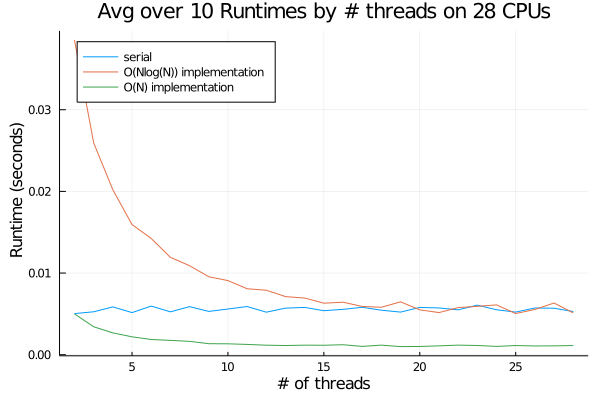
\includegraphics[scale=.45]{hw2_threads.png}
\end{figure}

\begin{figure}[h]
  \caption{}
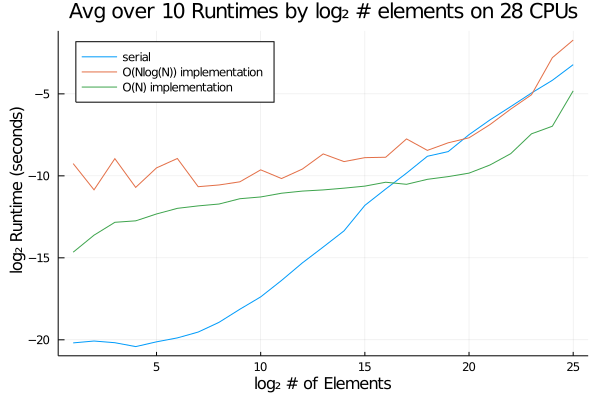
\includegraphics[scale=.45]{hw2_length.png}
\end{figure}

\end{document}
